\documentclass{article}
\usepackage[utf8]{inputenc}
\usepackage{hyperref}
\usepackage{natbib}
\usepackage{apalike}

\usepackage{graphicx}
\usepackage{subcaption}

%\usepackage{geometry}
%\usepackage[top=0.5in,bottom=1in,left=0.5in,right=0.5in]{geometry}

\title{Online News Popularity \\\large Bayesian Networks Assignment 1 --- Report}
\author{Thomas Churchman (s4206606) \& Jordi Riemens (s4243064)}
\date{December 12, 2016}

\begin{document}

\maketitle

\section{Problem Domain}
As people increasingly consume their news online, competition is fierce between the ever growing amount of news-related websites. This has sparked interest in applying data-driven methods to gain an edge over competing news outlets. For example, \citet{fernandes2015proactive} use various classification algorithms to predict---prior to publication---whether a given article would be popular on social media.

Far more interesting than merely predicting popularity, however, is using data-driven methods to gain insight into what makes articles popular. \citet{fernandes2015proactive} offers a method to better tailor written articles for social media shares, using stochastic hill climbing search methods to make suggestions, e.g. to change the amount of words in the title. However, rather than merely optimising given articles, we are interested in applying structural equation modelling to infer some of the mechanisms behind article popularity: which components of an article are relevant for popularity, and how are they related?


\section{Method}
Our project will use the ``Online News Popularity" data set, available on the UCI machine learning repository, which contains document news stories and their popularity published on \emph{Mashable}---a large news website.
The data consist of nearly all articles published on Mashable in two years, starting at January 7th 2013.
Only special occasion articles (with a different technical structure) were omitted.
All articles collected were older than 3 weeks to ensure the popularity measures would not be biased towards the end of the collection period.

The data have been preprocessed for use in computational models and consist of 48 features, with mixed feature types (nominal, integer, continuous ratio, and Boolean).
The features are of varying complexity. The low-level features require little pre-processing, such as the number of words present in the article.
A slightly higher-level feature, requiring some natural language processing, is the ratio of non-stop words in the text.
Some features stem from high-level models, such as the closeness of the text to latent topics found with LDA.
See Table~\ref{tab:table} for an overview of the dataset variables used.

As we have mainly numerical attributes, the straightforward implementation of a network in this domain is a Structural Equation Model (SEM), i.e. with linear Gaussian models. This includes coefficients between nodes, which indicate covariances between variables---a hint for the mechanisms behind news popularity we aim to examine. Furthermore, latent concepts explaining covariance of several variables at once can be introduced, which are of more theoretical interest.

We use the \texttt{lavaan} R package for Structural Equation Modelling for our implementation.
As linear models have been applied to this domain before in the context of classification \citep{petrovic2011rt}, non-linearity does not seem to be a necessity for explaining popularity in terms of features such as the ones in question here. 

\section{Data Pre-processing}
\subsection{Cleaning}
The data contain some abnormalities, and is cleaned by removing these.
One data point is an article with values above 1 on ratio variables that should be in a range of 0 to 1.
This data point is removed from the data.

Additionally, the data contain articles without text.
Though it is possible that articles without text occur naturally (e.g., articles with only images), these articles skew the distributions of many variables depending on word counts.
As such, all articles without text are removed.

\subsection{Transformations}

\begin{figure}
    \center
    \begin{subfigure}[t]{0.45\textwidth}
        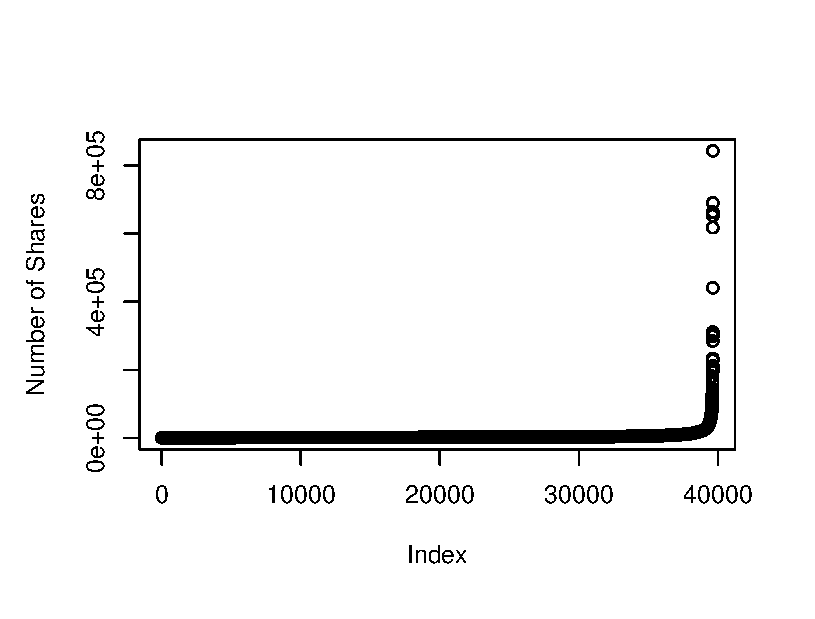
\includegraphics[width=\textwidth]{figs/zz-00-cumulative-plot-shares}
        \caption{Ordered plot of number of article shares for each article in the data set.}
    \end{subfigure}
    ~
    \begin{subfigure}[t]{0.45\textwidth}
        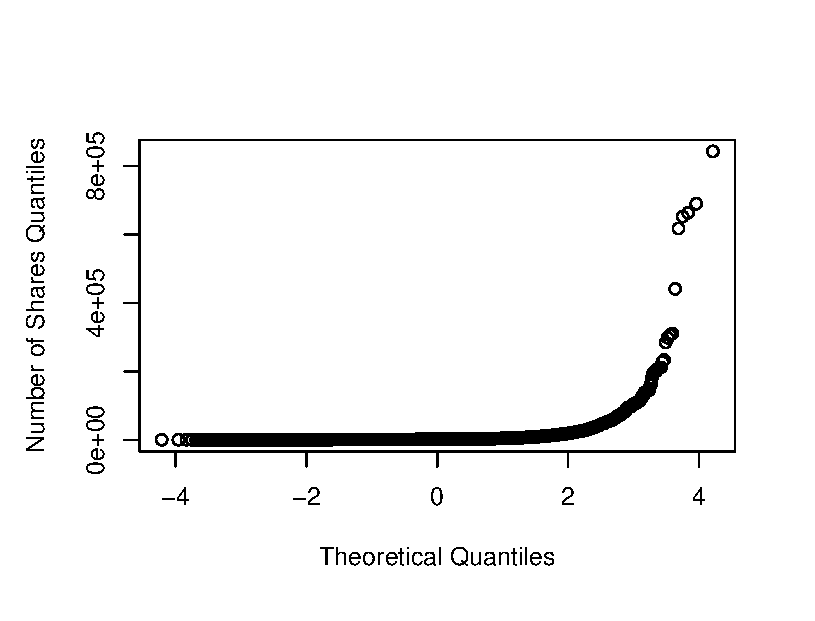
\includegraphics[width=\textwidth]{figs/zz-01-quantiles-number-of-shares}
        \caption{Quantile-Quantile plot for the distribution of article shares vs. the theoretical normal distribution of article shares.}
    \end{subfigure}
    
    \begin{subfigure}[t]{0.45\textwidth}
        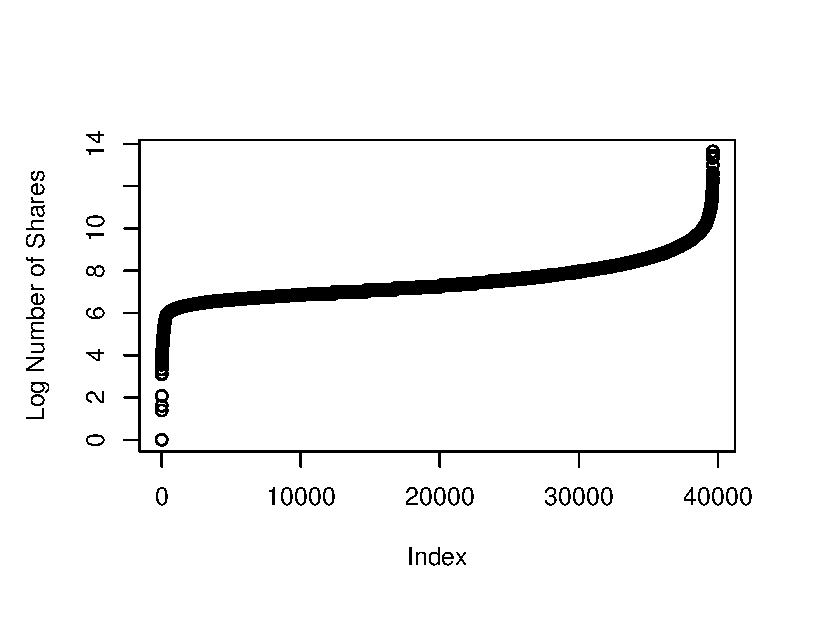
\includegraphics[width=\textwidth]{figs/zz-03-log-cumulative-plot-shares}
        \caption{Ordered plot of the log number of article shares for each article in the data set.}
    \end{subfigure}
    ~
    \begin{subfigure}[t]{0.45\textwidth}
        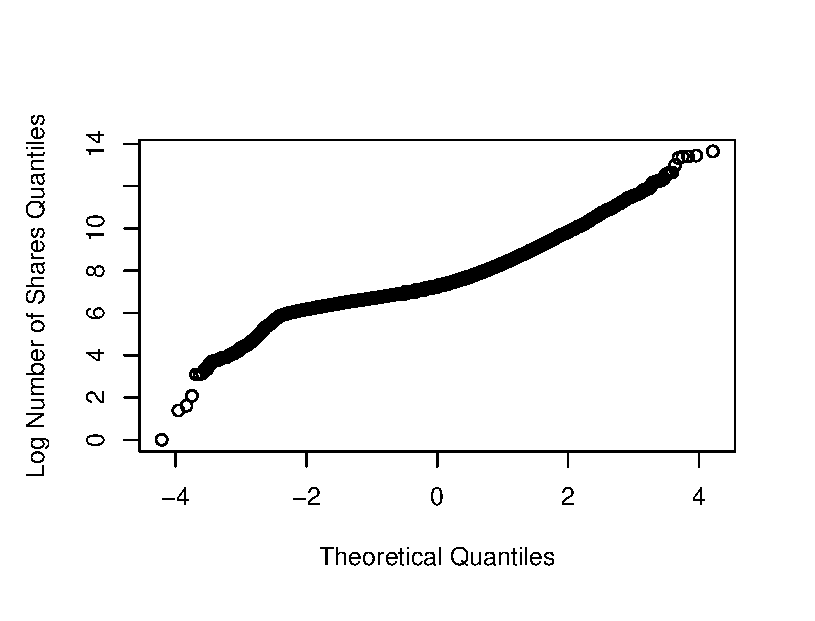
\includegraphics[width=\textwidth]{figs/zz-02-log-number-of-shares-quantiles}
        \caption{Quantile-Quantile plot for the distribution of log article shares vs. the theoretical normal distribution of log article shares.}
    \end{subfigure}
    
    \caption{Distribution of the number of article shares.}
    \label{fig:number_of_shares_distribution}
\end{figure}

The data contain variables with different distributions. For structural equation modeling with lavaan, it is assumed the data come from a normal distribution.
If the data are not normally distributed, the model fit space might not have a unique solution and identifying the correct model coefficients will be impossible.
As such, pre-processing steps have to be taken to ensure the data are suitable.

From Figures~\ref{fig:number_of_shares_distribution}(a) and~(b) it is clear the variable \emph{Number of 
Shares} has a heavy right skew.
Often, distributions with a heavy right skew are approximately exponential, and thus log-normal.
This would be expected for the number of shares relating to social networks, as is the case here: when one share reaches multiple people, the share count can be expected to grow exponentially.
By taking the log transform of this variable, it better approaches a normal distribution, as can be seen in Figures~\ref{fig:number_of_shares_distribution}(c) and~(d).

Other continuous variables approximately follow a normal or log-normal distribution, and the transform was taken on a per-variable basis by judging whether the transformed data better approximated a normal distribution.

\subsection{Normalization}
The data contain variables with different means and variances.
For ease of modelling, the (transformed) data are normalized to have 0 mean and unit variance.
Though in a structural equation model intercepts can be included, by having data with 0 mean this is no longer necessary.
Further, unit variance improves convergence, as iterative optimization is eased.

\subsection{Partitioning}
The data are partitioned into a fitting set containing 80\% of the observations and a testing set containing the remaining 20\%.

\section{Network Structure}

\begin{figure}
    \center
    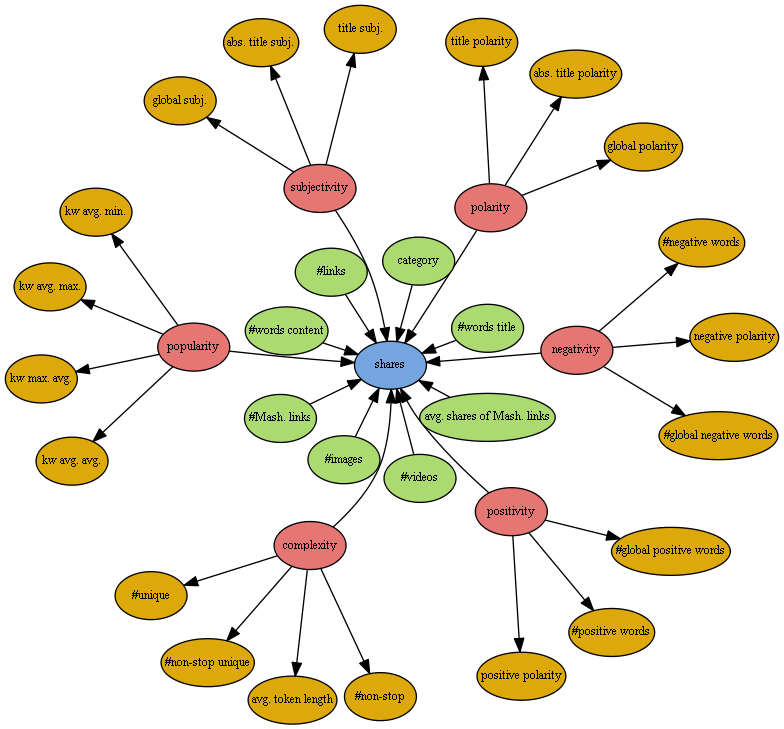
\includegraphics[width=\textwidth]{figs/network}
    \caption{The used network structure.}
    \label{fig:network}
\end{figure}

\subsection{General Structure}
Many variables in the data set used are naturally related, such as the rate of positive words and the rate of positive words among non-neutral words, or the average number of post shares within average keywords and the average number of post shares within popular keywords that the currently considered post is tagged with. Taking into account the large amount of variables even after discarding close to half the variables the original data set offers, some complexity control was in order.

To this end, we introduced latent concepts `summarising' several related observed variables, where possible. These include word complexity, involving word lengths as well as rates of non-stop and unique words; context popularity, comprising the average share counts of posts with shared keywords of differing popularity; as well as NLP-determined latent variables such as positivity and negativity, subjectivity and polarity of the article. Several more were considered, but proved impossible to fit, as is partly elaborated on below. These latent variables were then used as regressors for the log share count, along with some of the observed variables that were not involved in any latent concepts. The full network structure can be seen in Figure~\ref{fig:network}.


\subsection{Training Procedure}
\label{sec:training}
As mentioned above, several latent concepts proved impossible to fit, despite clearly having semantic meaning. These include straightforwardly untrainable two-factor concepts such as the link between the number of images and videos (both stemming from, for example, some variable `multimedia content'), which are fundamentally underspecified. However, a latent variable summarising the matches with the five LDA topic and one latent variable comprising the one-of-$k$-encoded article category variables also proved impossible to fit, likely due to their combination of extremely non-normal data with plausible negative covariances between all constituent observed variables (an article matching one topic or belonging to one category is less likely to match another topic well, and will not belong to any other category).

When putting the above general structure together in \texttt{lavaan}, however, one is faced with a multitude of errors, with the model often not being identified, or having a non-positive definite sample covariance matrix or implied covariance matrix between latent variables. Furthermore, negative implied latent and observed variable variances frequently occurred at least once in converged models. 

In the meeting with the course instructor, a two-step approach to training was suggested: fit each measurement model (defining one latent concept and its constituent observed variables) separately, predict the latent variable values for the observed data points, then fit a structural model in which latent concepts are related to the log share count and (possibly) each other. This divide makes each individual fit easier and helps convergence, as components that converge slowly can be isolated and cannot interfere with better-behaved parts of the network. However, it does limit the structure and power of the network, as covariances between observed variables require that their latent variables be fit together, and measurement models no longer have access to information relating to covariances between latent variables and the regression relation with the log share count.

\subsection{Improvements}
Apart from the $\chi^2$ measure on the model fits, we developed our model with inference in mind. Specifically, our target is to predict and explain the value of the log share count. Fortunately, this proved relatively simple in \texttt{lavaan}, as the regression coefficients could simply be read off from the model fits, and \texttt{lavaan} could predict latent variable values given observed variables. The coefficients and variable values can then be combined into an actual regression function predicting the log share count. The result can be compared with the actual log share count we try to model, giving metrics such as the mean absolute regression error.

When comparing the above two-step procedure with the earlier model, which contained all observed and latent variables together, it led to a significant decrease in both $\chi^2$ (which was halved) and the mean absolute regression error (which decreased by approximately a quarter). This indicates the two-step process does indeed help, although it is likely it particularly aids training and not so much modelling the true distribution.

However, this two-step procedure also limits any further improvements. Effectively we can still remove observed variables from latent variables, add them to another latent variable, or add them directly to the log share count's regression equation. We can also form new latent concepts. However, modelling covariances between latent variables or between observed variables can no longer influence the regression coefficients with the log share count without essentially reverting back to the overly large one-step model; they can only influence the $\chi^2$ measure on the fit (although they can majorly affect this statistic, at least). 

\section{Conclusion}
\subsection{Metrics}
As the second step in the final two-step model only consisted of a regression, it has a $\chi^2$ of 0 (the sum of $\chi^2$ for the two measurements models with a latent measured by more than three factors is 11,165).
The model's inference performance was tested on the held-out test set.
On this set, the mean absolute error on log scale of the share prediction was $0.695$ (translating to being off by a factor 2 on average).
A baseline model taking the mean of the dataset as predictor achieves a prediction error of $0.761$.
The two-step model has a better performance, but not by a huge amount, which is slightly disappointing.

Rearranging observed variables between latent concepts, or bringing them out of concepts into the main regression equation, too proved to have only minuscule effects on the regression error, in the order of $0.1\%$, although again the $\chi^2$ could undergo significant changes as a result of these rearrangements. Thus, it seems like this is the limit of the combination of this type of model and data set, and further significant improvements in terms of regression error within this particular framework seem unlikely.

\subsection{Insights}
Despite the discouraging numeric results described above, the project is not wholly unsuccessful. In particular, thanks to the two-step training procedure, the regression coefficients could be examined efficiently. \texttt{lavaan} also performs some rudimentary hypothesis testing on these regression coefficients, indicating which correlations it finds to be significant, although the large number of $p=0.000$ results casts some doubt on the validity of the exact numbers found here. Nevertheless, insights could be gained by examining the stronger among these links (very high regression coefficients compared to their standard deviations).

The one factor that seems very predictive for popularity of an article in question is `context popularity'. This refers to two things. The first part of this category refers to a single observed variable, namely the average log number of shares of other Mashable articles the current article links to. Secondly, posts are tagged with keywords hinting at the article's contents, and popularity measures can be associated to keywords themselves---some topics are more popular than others, and this is not measured optimally by a coarse-grained category such as \emph{lifestyle}, \emph{social media} or \emph{tech}. Articles that are a part of popular keywords are likely to be popular, too. Together, these two factors can account for a $30\%$ increase in number of shares per standard deviation of these factors.

Coincidentally, this provides us with a good example of the difference between association and causation. It does not follow from the relations laid out above that merely adding more links to popular articles, or misrepresenting the keywords of an article, will increase that article's popularity. Strictly speaking it does not even follow that writing an article such that it truly has certain keywords will cause it to have high popularity. The joint distribution between two variables (such as the average share count of links in this article and this article's share count) does not tell us how that distribution ought to change if external conditions were to change, such as from observational to manipulatory setup.

Although keywords are more predictive than coarse-grained categories, the coarse-grained category does in fact matter. It appears that articles in the social media category are shared the most, whereas articles in the world and entertainment categories are shared far less (there is approximately a $67\%$ difference in number of shares between these categories).

This might suggest that, as long as one chooses their topic well, their article has a higher chance of becoming popular. Strictly speaking this cannot be inferred, as it is possible, but perhaps less likely, that unobserved external factors such as recent events cause both categories and popularity, thereby fully explaining the association between these two variables. There are additional factors that appear to significantly contribute to article popularity in our model. For one, an interesting effect appears in the usage of links in articles. The log number of links to external sites seems to lead to an increase in number of shares ($10\%$ increase per standard deviation), perhaps indicating either well-sourced articles or articles that point to interesting sites are popular. On the contrary, the same statistic for links within Mashable has the opposite sign: using more links to Mashable articles in a new Mashable article seems to decrease the number of shares. This could be interpreted as a dislike towards self-advertising, or in a more positive light that people like to use Mashable as a `front page of the internet' (such as the social news aggregation site \emph{Reddit} calls itself), and use it more to find other interesting sites than to browse Mashable news itself.

Apart from this, it seems writing style also has an impact on the popularity of a news article. Complexity, understandably, negatively affects an article's popularity, although this has a relatively small effect ($4\%$ decrease per standard deviation). Conversely, the use of images and videos in the article seems to have the opposite effect ($8\%$ increase in shares per standard deviation of both). This reinforces the belief that people treat Mashable as a front page of the internet, using it to find not only interesting websites as above, but also interesting pictures and videos, rather than just to read news (let alone complicated articles).

Unfortunately, the NLP statistics such as polarity and subjectivity, have a very small effect, if any. If, in reality, these properties of an article do have an effect on its popularity, the effect might not be evident from our analyses due to the fact they have not been perfected yet, and measure only weakly the quantity of interest. Similarly, it is important to note that factors other than the ones used here, perhaps not even measurable at all (e.g. timeliness, novelty, creativeness), might have an effect on something as complex as an article's popularity, and the existence of these factors might also have an adverse effect on our model's performance.

\bibliographystyle{apalike}
\bibliography{bibliography}

\appendix

\begin{table}
    \centering
    \begin{tabular}{|p{0.5\linewidth}|p{0.15\linewidth}|r|}
        \hline
        \textbf{Feature} & \textbf{Type} & \textbf{Levels / Range}
        \\
        \hline
        \multicolumn{3}{|c|}{\textbf{Words}}
        \\
        \hline
        Number of words in the title & numerical & 2 -- 23
        \\
        \hline
        Number of words in the article & numerical & 18 -- 8474
        \\
        \hline
        Average word length & numerical & 3.6 -- 8.04
        \\
        \hline
        Rate of non-stop words & numerical & 0.99 -- 1
        \\
        \hline
        Rate of unique words & numerical & 0.11 -- 1
        \\
        \hline
        Rate of unique non-stop words & numerical & 0.12 -- 1
        \\
        \hline
        \multicolumn{3}{|c|}{\textbf{Links}}
        \\
        \hline
        Number of links & numerical & 0 -- 304
        \\
        \hline
        Number of Mashable article links & numerical & 0 -- 116
        \\
        \hline
        Average number of shares of Mashable links & numerical & 0 -- 843,300
        \\
        \hline
        \multicolumn{3}{|c|}{\textbf{Digital Media}}
        \\
        \hline
        Number of images & numerical & 0 -- 128
        \\
        \hline
        Number of videos & numerical & 0 -- 91
        \\
        \hline
        \multicolumn{3}{|c|}{\textbf{Time}}
        \\
        \hline
        Published in a weekend & categorical & 2 levels
        \\
        \hline
        \multicolumn{3}{|c|}{\textbf{Keywords}}
        \\
        \hline
        Mean average number of shares of articles in keywords & numerical & 0 -- 43,567.67
        \\
        \hline
        Average max. number of shares of articles in keywords & numerical & 0 -- 298,400
        \\
        \hline
        Average number of shares of articles in the best keyword & numerical & 0 -- 843,300
        \\
        \hline
        Average number of shares of articles in the worst keyword & numerical & 0 -- 42,827.86
        \\
        \hline
        Article category & categorical & 6 levels
        \\
        \hline
        \multicolumn{3}{|c|}{\textbf{Natural Language Processing}}
        \\
        \hline
        Closeness to top 5 LDA topics & numerical (5 features) & 0.02 -- 0.93
        \\
        \hline
        Title subjectivity & numerical & 0 -- 1
        \\
        \hline
        Article text subjectivity score & numerical & 0 -- 1
        \\
        \hline
        Title sentiment polarity & numerical & -1 -- 1
        \\
        \hline
        Rate of positive and negative words & numerical (2 features) & 0 -- 0.18
        \\
        \hline
        Positive and negative words rates among non-neutral words & numerical (2 features) & 0 -- 1
        \\
        \hline
        Average polarity of positive and negative words & numerical (2 features) & -1 -- 1
        \\
        \hline
        Article text polarity score & numerical & -0.39 -- 0.73
        \\
        \hline
        \multicolumn{3}{|c|}{\textbf{Metric}}
        \\
        \hline
        Number of article shares & numerical & 1 -- 843,300
        \\
        \hline
    \end{tabular}
    \caption{The used features of the data set after cleaning the data, before transformation and normalization of the values.}
    \label{tab:table}
\end{table}

\end{document}
